\section{Training Dynamics and the Neural Tangent Kernel}
\label{sec:Training}

Having defined the physical context of this work and established some properties
of the neural network at initialisation, we now turn to the optimisation
process. In the context of machine learning, specifically when dealing with
neural networks, optimisation is an iterative algorithm that updates the
parameters of the network in order to minimise a figure of merit defined
appropriately. Due to the large number of parameters that characterise a neural
network, the figure of merit (also known as \textit{error function},
\textit{loss function}, or simply \textit{loss}) is a non-convex
high-dimensional function that poses a challenge in the minimisation task. In
addition, in order to avoid \textit{over-} and \textit{under-learning}, these
training algorithms are paired with the so-called \textit{stopping criterion},
which specifies the optimal condition to end the training process.

In practice, this task is tackled by using gradient methods where the direction
towards the minimum is characterised by the gradient of the loss function. These
methods are usually improved by including, for instance, stochasticity and
information on previous iterations. A detailed overview of these extended
gradient methods is beyond the scope of this work. In the context of PDF
determinations, the NNPDF collaboration makes intensive use of these tools and
the reader is encouraged to refer to Ref.~\cite{NNPDF:2021njg} for an extensive
discussion.

Our main aim in this paper is understanding the dynamics driving the training
process. Indeed, while these algorithms have achieved remarkable empirical
success, a theoretical understanding of the optimization process remains
elusive. Therefore, we work in a simplified setting where we consider the
simplest gradient method, \textit{i.e.} Gradient Descent (GD). Furthermore, we
will consider a dataset for which predictions can be computed using one flavour
combination in the PDFs, so that the integral in Eq.~\eqref{eq:TheoryPred}
reduces to
\begin{equation}
    \label{eq:TheoryPredSingleFlav}
    T_I[f] = \int dx\, C_{I}(x) f(x)\,.
\end{equation}
The details of the dataset and the definition of the flavour combination
considered in this work are provided in Appendix~\ref{app:dataset}.
For simplicity, we do not implement cross-validation or stopping
criteria\footnote{ We are aware that such a framework has limited applicability
in the context of PDF determination, and we are far from assuming this as an
optimal choice. Again, the focus remains on the methodological aspects rather
than the underlying physics.}. Extensions to theoretical predictions that are
quadratic in the PDFs, multiple flavour combinations, alternative minimizers,
and cross-validation tools are left for future work.

Finally, we emphasise that the results in this sections, while obtained having in mind
neural networks, apply to any fixed parametrisation, including polynomials or
kernels~\cite{Costantini:2025wxp}.

\subsection{Training in Functional Space}
\label{sec:GradFlow}

For analytical tractability, GD is described as a continuous flow of the
parameters $\theta$ in training time $t$ along the negative gradient of the loss
function $\mathcal{L}$. For sufficient small learning rates, this continuous
flow approximates the discrete GD trajectory in parameter space, as extensively
discussed in Ref.~\cite{barrett2022igr}. The continuous Gradient Flow (GF) is
then given by
\begin{align}
    \label{eq:GradientFlowDef}
    \ddt &\theta_{t,\mu} = -\nabla_\mu \mathcal{L}_t\, ,
\end{align}
where $\theta_{t,\mu}$ and $\mathcal{L}_t$ identify respectively the parameter
and the loss function at training time $t$. We focus here on quadratic loss
functions that are obtained as the negative logarithm of Gaussian data
distributions around their theoretical predictions,
\begin{align}
    \label{eq:QuadLoss}
    \mathcal{L}_t = \frac12 \left(Y - T[f_t]\right)^T C_Y^{-1} \left(Y - T[f_t]\right)\, ,
\end{align}
where $f_t$ is the output of the network at training time $t$, which follows
from the time-dependence of the internal parameters. Here $C_Y$ is the
covariance of the data, which includes statistical and systematic errors given
by the experiments and also any theoretical error, like \eg\ missing higher
orders in the theoretical predictions. Indices that are summed over are
suppressed to improve the clarity of the equations. Note that the loss function
at training time $t$ is computed using the theoretical prediction $T[f_t]$, \ie\
the result of Eq.~\eqref{eq:TheoryPred} computed using the fields at training
time $t$. For a quadratic loss, the gradient is
\begin{align}
    \nabla_\mu \mathcal{L}_t = - \left(\nabla_\mu f_t\right)^T \left(\frac{\partial T}{\partial f}\right)_t
      C_Y^{-1} \epsilon_t\, ,
\end{align}
where, writing explicitly the data index,
\begin{align}
    \label{eq:EpsDef}
    \epsilon_{t,I} = Y_I - T_I[f_t]\, , \quad I=1, \ldots, \ndat\, .
\end{align}
For the specific case of a quadratic loss function, the gradient is proportional
to $\epsilon_t$, which is the difference between the theoretical prediction and
the data at training time $t$. If at some point during the training the
theoretical predictions reproduce all the data, the training process ends. 

A further simplification is obtained in the case of data that depend linearly on
the unknown function $f$. In the specific case of NNPDF fits, the integrals in
Eq.~\eqref{eq:TheoryPred} are approximated by a Riemann sum over the grid of $x$
points,
\begin{align}
    \label{eq:FKTabDef}
    T_I[f] \approx \sum_{i=1}^{\nflav}\sum_{\alpha=1}^{\ngrid} \FKtab_{Ii\alpha} f_{i\alpha}\, ,
\end{align}
and hence
\begin{align}
    \label{eq:dTbydf}
    \left(\frac{\partial T_I}{\partial f_{i\alpha}}\right)_t =
        \FKtab_{Ii\alpha}\, ,
\end{align}
which is independent of $t$. With simple algebraic steps, the flow of parameters
$\theta$ can be translated into a flow for the fields,
\begin{align}
    \label{eq:NTKFlow}
    \ddt &f_{t,i_1\alpha_1} = (\nabla_\mu f_{t,i_1\alpha_1}) \ddt \theta_\mu =
      \Theta_{t,i_1\alpha_1i_2\alpha_2}
      \FKtabT_{i_2\alpha_2I} \left(C_Y^{-1}\right)_{IJ} \epsilon_{t,J}\, ,
\end{align}
where we have defined the Neural Tangent Kernel~\cite{jacot2018neural}
\begin{align}
    \label{eq:NTKDef}
    \Theta_{t,i_1\alpha_1i_2\alpha_2} = \sum_\mu
    \nabla_\mu f_{t,i_1\alpha_1} \nabla_\mu f_{t,i_2\alpha_2}\, .
\end{align}
As it will become clearer later, the NTK provides a powerful framework for
understanding neural network dynamics during training. Originally developed by
Jacot et al.~\cite{jacot2018neural} to analyse infinite-width feed-forward
networks, the NTK theory has since been extended to diverse architectures
including convolutional networks~\cite{arora2019exact} and recurrent
networks~\cite{alemohammad2021recurrent}. This theoretical framework has proven
invaluable for characterizing learning dynamics and generalization properties
across various network designs. We will see in the following and in
Sec.~\ref{sec:LazyTraining} how the NTK can provide useful insights also in the
context of PDF fitting.

In order to facilitate the discussion in Sec.~\ref{sec:Lazy},
Eq.~\eqref{eq:NTKFlow} can be rewritten in a more compact form. We first omit
the indices such that, for instance,
\begin{align}
  \left(\frac{\partial T}{\partial f}\right)_t = \FKtab\, , \quad
  \Theta_t = \left(\nabla_\mu f_t\right) \left(\nabla_\mu f_t\right)^T\, .
  \label{eq:dTdfForLinearObs}
\end{align}
Then, using the definition of the error in Eq.~\eqref{eq:EpsDef}, we can rewrite
Eq.~\eqref{eq:NTKFlow} as follows
\begin{align}
    \label{eq:FlowEquationNoIndices}
    \ddt f_t = -\Theta_t M f_t + b\, ,
\end{align}
where
\begin{align}
    M &= \FKtabT C_Y^{-1} \FKtab\, , \quad b_t = \Theta_t \FKtabT C_Y^{-1} Y\, .
    \label{eq:MandBDef}
\end{align}
Here $M$ is a positive-semidefinite matrix that depends only on the data and the
theoretical predictions, while $b$ is a vector that depends also on the data.

Before moving to the next subsection, a few comments comments are in order.
First, although derived in the context of neural networks, these equations do
not refer to a specific parameterization. Indeed, these remain valid even when
an explicit functional form to parametrize the PDFs is chosen, as \eg~in
Refs.~\cite{Bailey:2020ooq,Hou:2019efy,Costantini:2025wxp}. Second, it is
interesting to observe that the flow equation,
Eq.~\eqref{eq:FlowEquationNoIndices}, depends on two matrices, $\Theta$ and $M$.
The former encodes the model dependence, while the latter contains the physical
information. The interplay between these two matrices is crucial for
understanding the training dynamics, as it will be discussed in
Sec.~\ref{sec:NTKAlign}. Finally, the NTK derived in Eq.~\ref{eq:NTKDef} is
inherently time-dependent in a complex way, which precludes any attempt at
integrating Eq.~\ref{eq:FlowEquationNoIndices} analytically. We will come back
to this point in Sec.~\ref{sec:Lazy}, and we now discuss the properties of the
NTK during training.

\subsection{Inside the Training Dynamics: an NTK perspective}

From Eqs.~\eqref{eq:NTKDef} and~\eqref{eq:FlowEquationNoIndices}, we observe
that the NTK encodes the dependence on the architecture of the network and
governs its training dynamics. The analysis of the NTK properties is thus
crucial for understanding the behaviour of the network during training. We first
discuss the properties of the NTK at initialisation, before moving to the
training phase, where we provide a detailed study of the NTK in the context of
the NNPDF methodology.

% ===================================
\begin{figure}[t!]
  \centering
  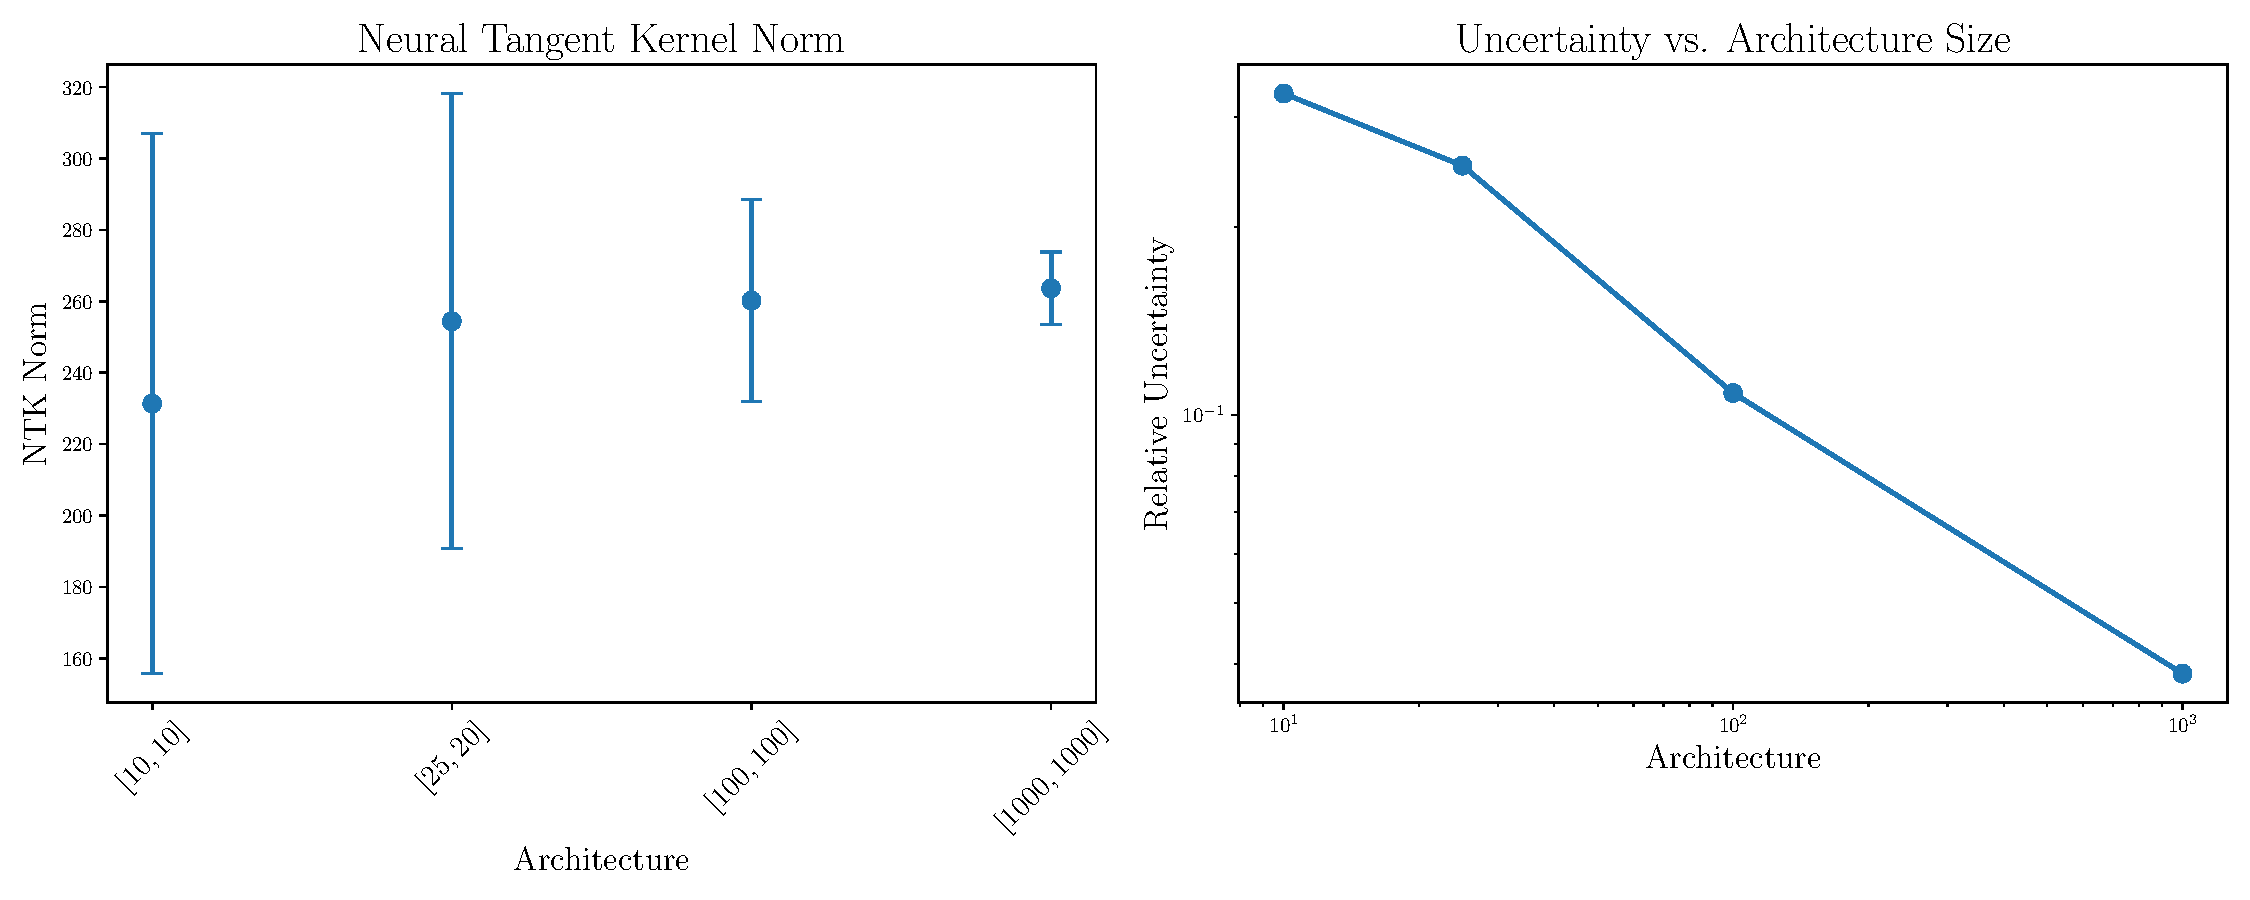
\includegraphics[width=0.90\textwidth]{figs/section_3/ntk_initialization_with_uncertainty.pdf}
  \caption{Frobenius norm of the NTK at initialisation, $\lVert \Theta_0
  \rVert$, in function of the width of the network. On the left, the central
  values and uncertainty bands are obtained as the mean and one-sigma deviation
  of the ensemble of networks. The plot on the right shows the relative
  uncertainty.}
  \label{fig:NTKInit}
\end{figure}
% ===================================

\subsubsection{NTK at initialisation}
\label{sec:NTKAtInit}

Before training, the NTK is blind to data and depends on the $x$-grid of input
and on the architecture, as it can be seen from Eq.~\eqref{eq:NTKDef}. The NTK
is a function of the fields $f$, which are stochastic variables described by
their joint probability distribution as discussed in Sect.~\ref{sec:Init}.
Therefore the NTK is also a stochastic variable, with its own probability
distribution, which we represent as usual as a set of replicas. 

It is argued in the literature that, in the large-width limit, the variance of
the NTK over the set of replicas tends to zero with the width of the hidden
layers (see, \textit{e.g.}, \cite{Roberts:2021fes}). In order to quantify the
variation of the NTK, we start by computing the Frobenius norm of the NTK over
an ensemble of networks for different architectures. For each architecture, we
consider the mean value and standard deviation of the norm as statistical
estimators of the variations of the NTK. The result is displayed in
Fig.~\ref{fig:NTKInit}. Even though the Frobenius norm is a coarse indicator of
the variations of the NTK, the figure shows clearly that the variance of the
norm becomes smaller with the size of the network, which is consistent with the
theoretical expectation that the NTK should not fluctuate for infinite-width
networks\footnote{Note that, in addition to the scaling $\mathcal{O}(1/n)$
theoretically predicted for large networks, the uncertainty bands include
bootstrap errors due to the finite size of the ensemble. Using an ensemble of
100 replicas, the bootstrap error on the standard deviation is $\sim 10\%$.}.

% ===================================
\begin{figure}[t]
  \centering
  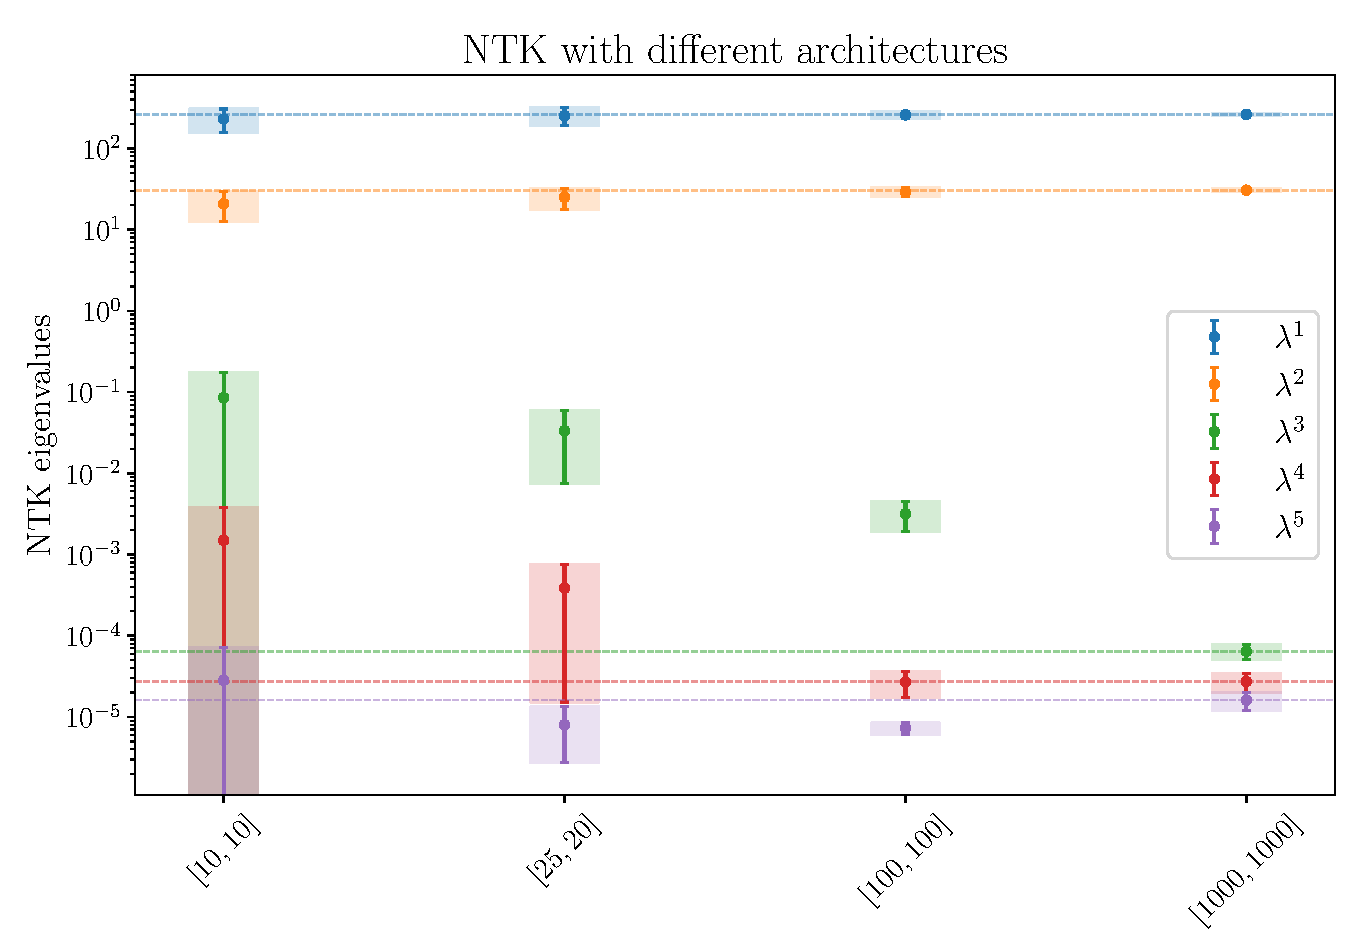
\includegraphics[width=0.45\textwidth]{figs/section_3/ntk_initialization_arch.pdf}
  \caption{Spectrum of the NTK at initialisation for the architectures shown in
  Fig.~\ref{fig:NTKInit}. Error bands correspond to one-sigma uncertainties over
  the ensemble of networks.}
  \label{fig:NTKSpectrum}
\end{figure}
% ===================================

A more quantitative description of the NTK at initialisation is provided by its
spectrum, which is shown in Fig.~\ref{fig:NTKSpectrum} for four different
architectures. Inspecting the figure, we see that the spectrum of the NTK is
heavily hierarchical, and only few eigenvalues are actually
non-zero\footnote{Note that, due to the large difference in magnitude of the
eigenvalues, the finite precision used in our codes introduces noise in the
decomposition, so that small eigenvalues should be effectively considered zero.
We discuss the cut-off tolerance in Appendix~\ref{app:cutoff}.}. This means that
only a small subset of active directions can inform the network during training,
as it will be discussed later. Note that, at least at initialisation, these
observations do not depend on the architecture. The eigenvalues in
Fig.~\ref{fig:NTKSpectrum} are mostly independent of the size of the network.
There is a downward fluctuation of the third eigenvalue for the largest
architecture that we considered, but we do not have any evidence that this drop
is a physical feature of the system, rather than a fluctuation. Finally, the
variance of the set of eigenvalues over replicas decreases with increasing size,
as expected. 

% \FloatBarrier

\subsubsection{NTK During Training}
\label{sec:NTKDuringTraining}

We now discuss the behaviour of the NTK during training. To this end, we are
going to adopt the so-called {\em closure tests} developed by the NNPDF
collaboration. A closure test uses synthetic data, generated using a known set
of PDFs, to train the neural network. The PDFs used for generating the data are
called here {\em input}\ PDFs. The results of the training are then compared to
the known input PDFs; the performance of the training algorithm and the NN
architecture are assessed by quantifying the comparison between trained PDFs and
input PDFs. Following the original presentation in Ref.~\cite{NNPDF:2014otw}, we
distinguish three levels of closure tests, which are defined by the complexity
of the data used to train the NNs. We use the standard NNPDF nomenclature and
refer to these three levels as level-0 (L0), level-1 (L1), and level-2 (L2)
closure tests, and we denote the input PDFs used to generate the data as $\fin$.
The definitions of these three levels of data are given in Appendix~\ref{app:dataset}.

For each of the closure-test data given above, we perform a fit of the
non-single triplet combination $T_3$ using the NNPDF methodology. To do so, we
initialise an ensemble of $\nreps = 100$ replicas with identical architecture,
training each replica independently using GD optimization. Throughout the
training process, we track the evolution of the NTK to understand how the
network's effective dynamics change as it learns the target function.

\paragraph{Onset of Lazy Training} 
% ===================================
\begin{figure}[t]
  \centering
  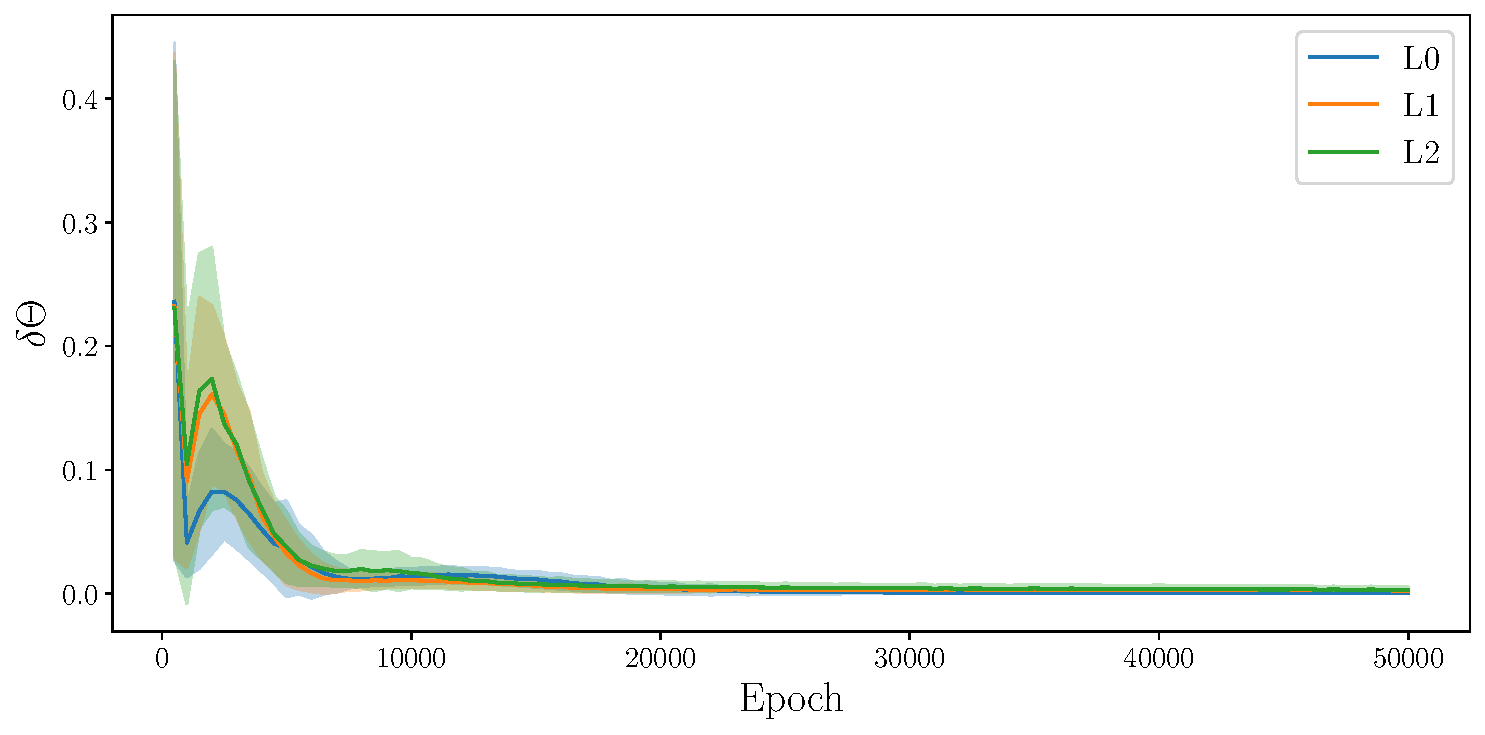
\includegraphics[width=0.60\textwidth]{section_3/delta_ntk.pdf}
  \caption{Relative variation of the NTK during training for L0, L1, and
  L2 data. Error bands correspond to one-sigma uncertainties over the ensemble
  of networks.}
  \label{fig:NTKTime}
\end{figure}
% ===================================

% ===================================
\begin{figure}[t]
  \centering
  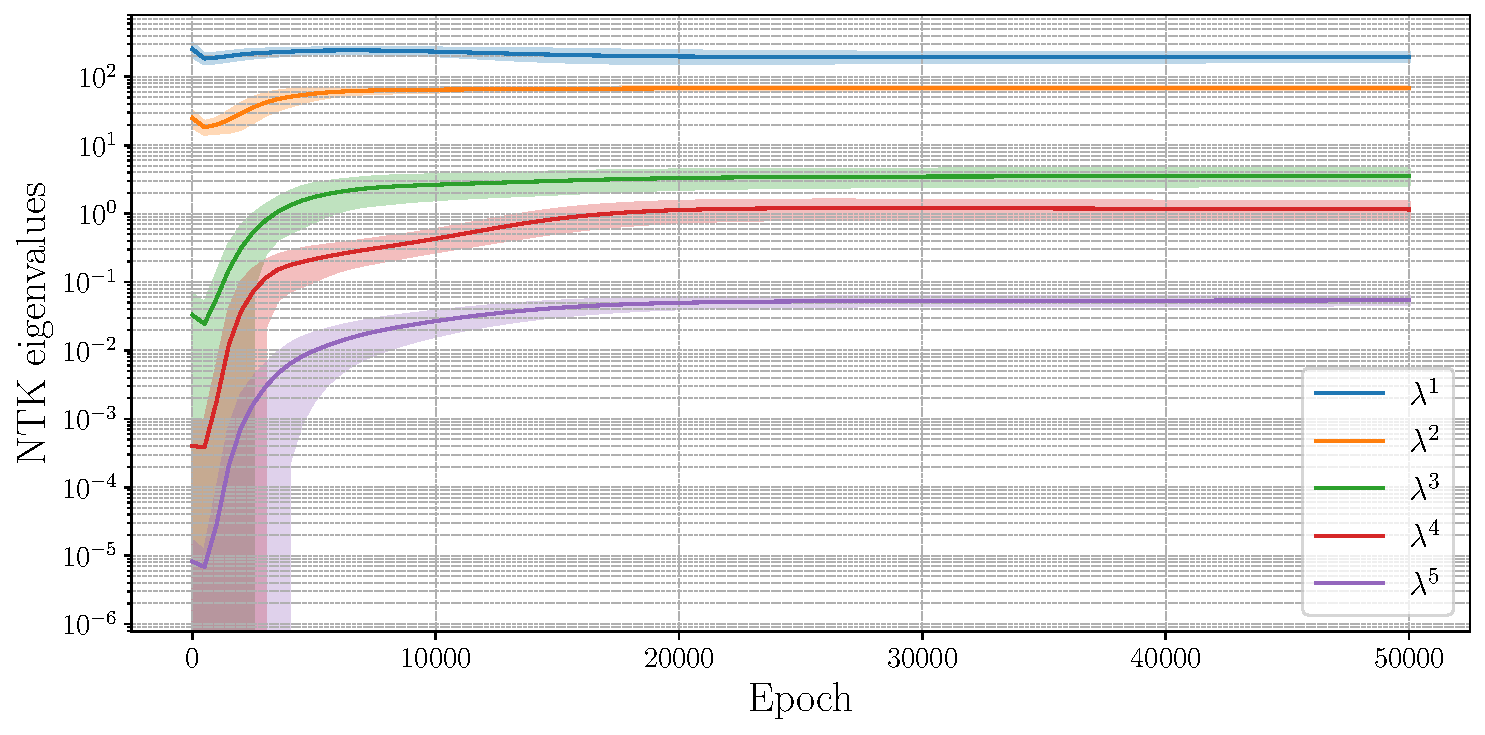
\includegraphics[width=0.3\textwidth]{section_3/ntk_eigvals_single_plot_L0.pdf}
  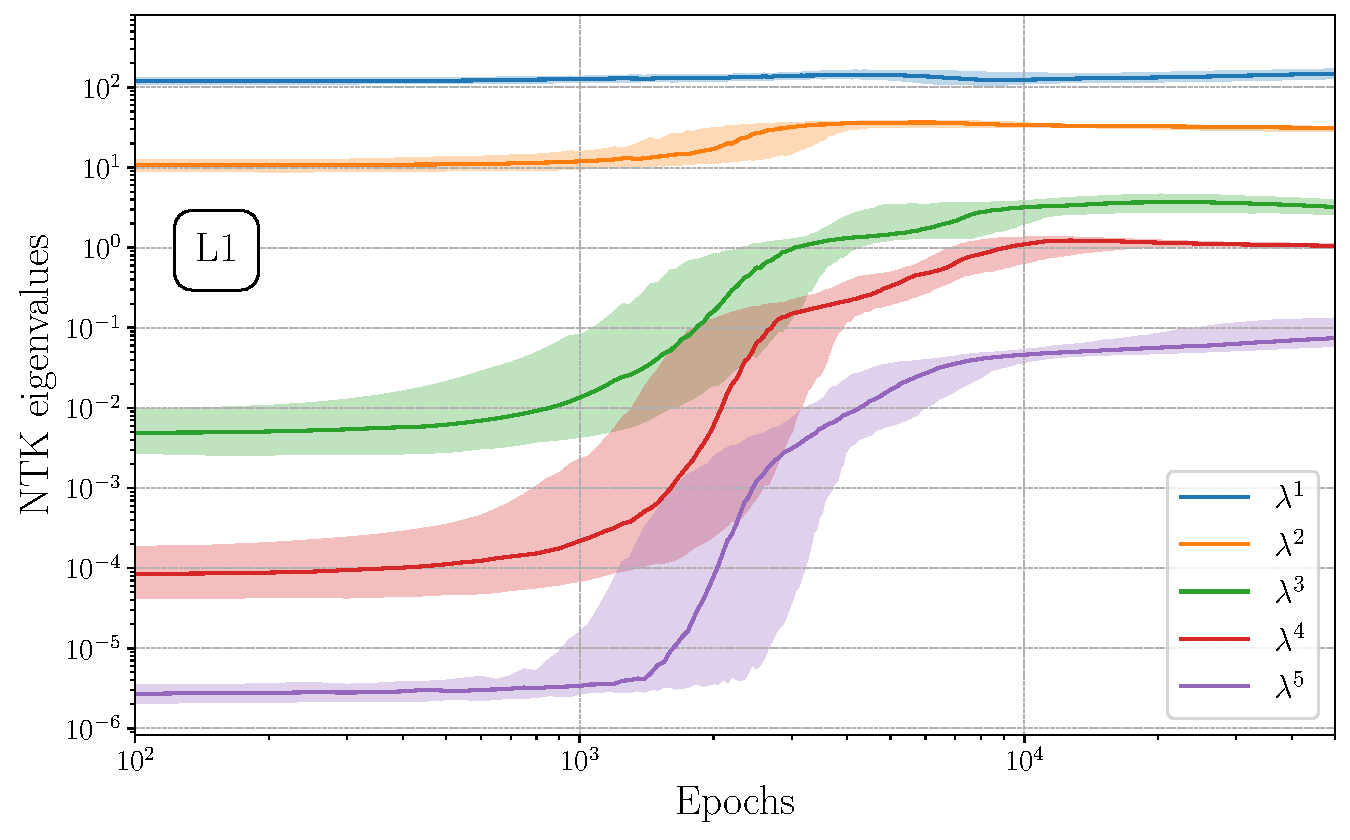
\includegraphics[width=0.3\textwidth]{section_3/ntk_eigvals_single_plot_L1.pdf}
  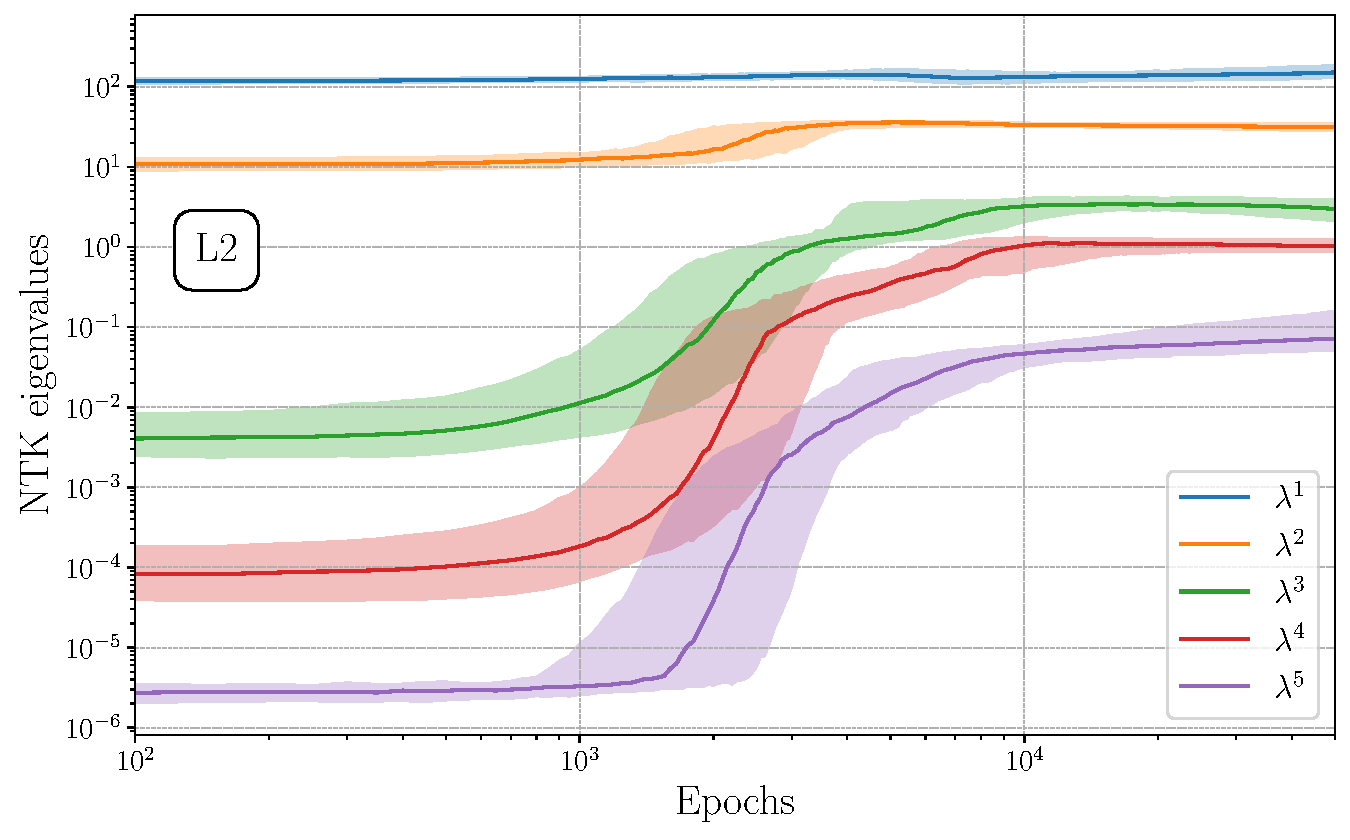
\includegraphics[width=0.3\textwidth]{section_3/ntk_eigvals_single_plot_L2.pdf} 
  \caption{Evolution during training of the first five eigenvalues of the NTK
  using L0 (left), L1 (center), and L2 (right) data. Solid lines represent the
  median over the ensemble of networks, while solid bands correspond to 68\%
  confidence level.}
  \label{fig:NTKEigvalsTime}
\end{figure}
% ===================================

As a first estimator of the variation of the NTK, we show in
Fig.~\ref{fig:NTKTime} the Frobenius norm of the variation during training,
normalized by the Frobenius norm of the NTK itself, 
\begin{equation}
\delta \Theta_t = \frac{\lVert \Theta_{t+1} - \Theta_t \rVert}{\lVert \Theta_t \rVert} \;,
\label{eq:DeltaNTK}
\end{equation}
for the three different datasets, L0, L1, and L2. Inspecting the plot reveals that
the NTK undergoes significant changes during the initial phase of training, with
the relative variation $\delta \Theta_t$ reaching values as high as $6\%$. This
indicates that our settings differ from the standard picture of lazy training in
the context of very wide networks, as discussed \eg~in
Refs.~\cite{jacot2018neural,Roberts:2021fes,lee2019wide}. Remarkably, we do not
observe a dependence on how data have been generated, indicating that the NTK is
able to learn across the noise that affects the data. 

After this initial phase -- corresponding approximately to the first 20,000
epochs in our experiment -- the NTK tends to stabilize. These two regions will
be referred to as the \textit{rich} and \textit{lazy} training regimes,
respectively, in keeping with the standard terminology adopted in the literature
(see, \eg Ref.~\cite{fort2020dlvk} where two similar regimes where also
identified). We do not comment any further on the implications of the lazy
regime, and postpone the discussion to Sec.~\ref{sec:Lazy}.

\FloatBarrier

\paragraph{Eigenvalues During Training}

Further insight on the evolution of the NTK can be obtained by studying its
eigensystem as a function of the training time. In Fig.~\ref{fig:NTKEigvalsTime}
we report the variation of the first five eigenvalues of the NTK, using the
standard NNPDF architecture, for L0, L1, and L2 data. We see that the
hierarchical structure observed at initialisation is preserved, but the size of
the subdominant eigenvalues increases significantly in the early stages of
training -- by one or two orders of magnitude depending on the specific
eigenvalue. 

% ===================================
\begin{figure}[t]
  \centering
  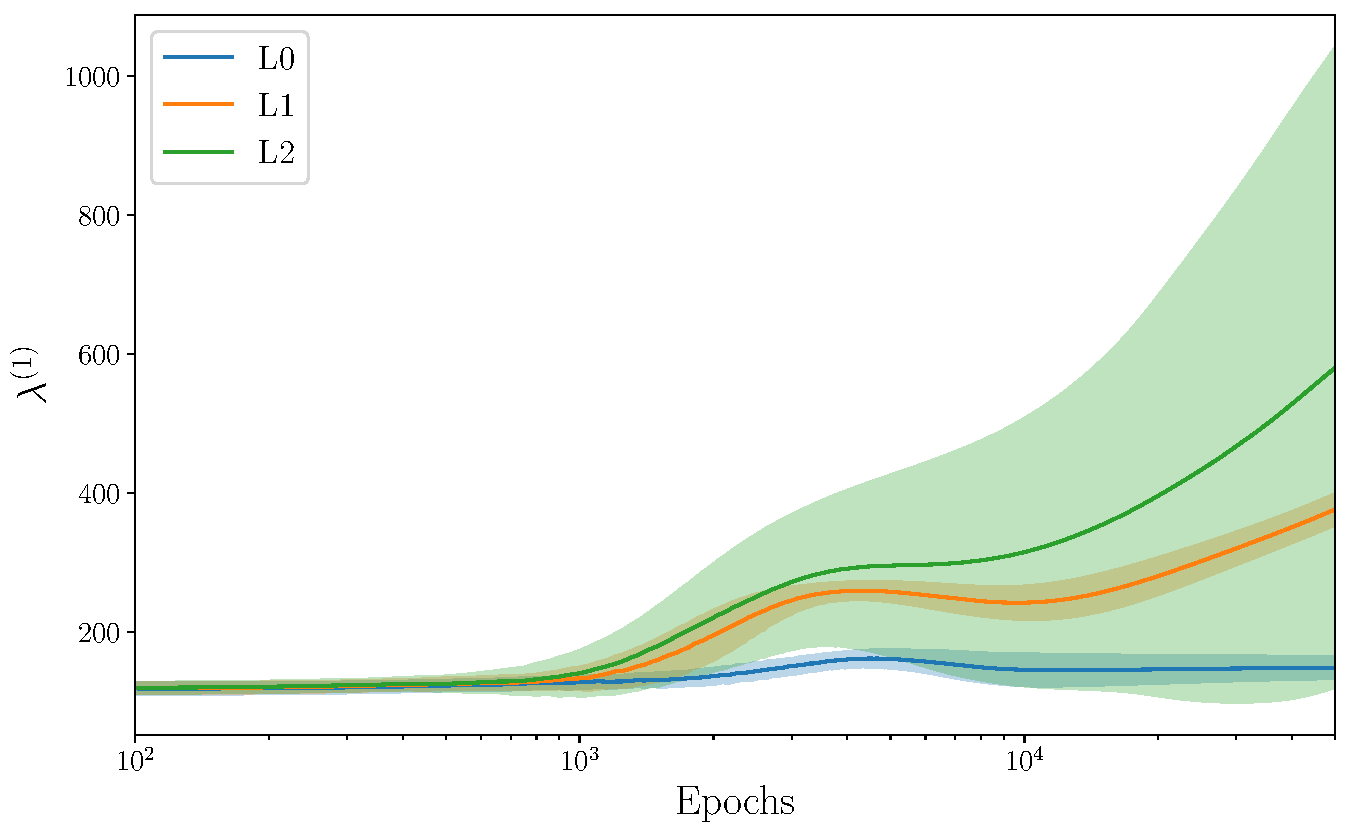
\includegraphics[width=0.30\textwidth]{figs/section_3/ntk_eigvals_L0_L1_L2_n_1.pdf}
  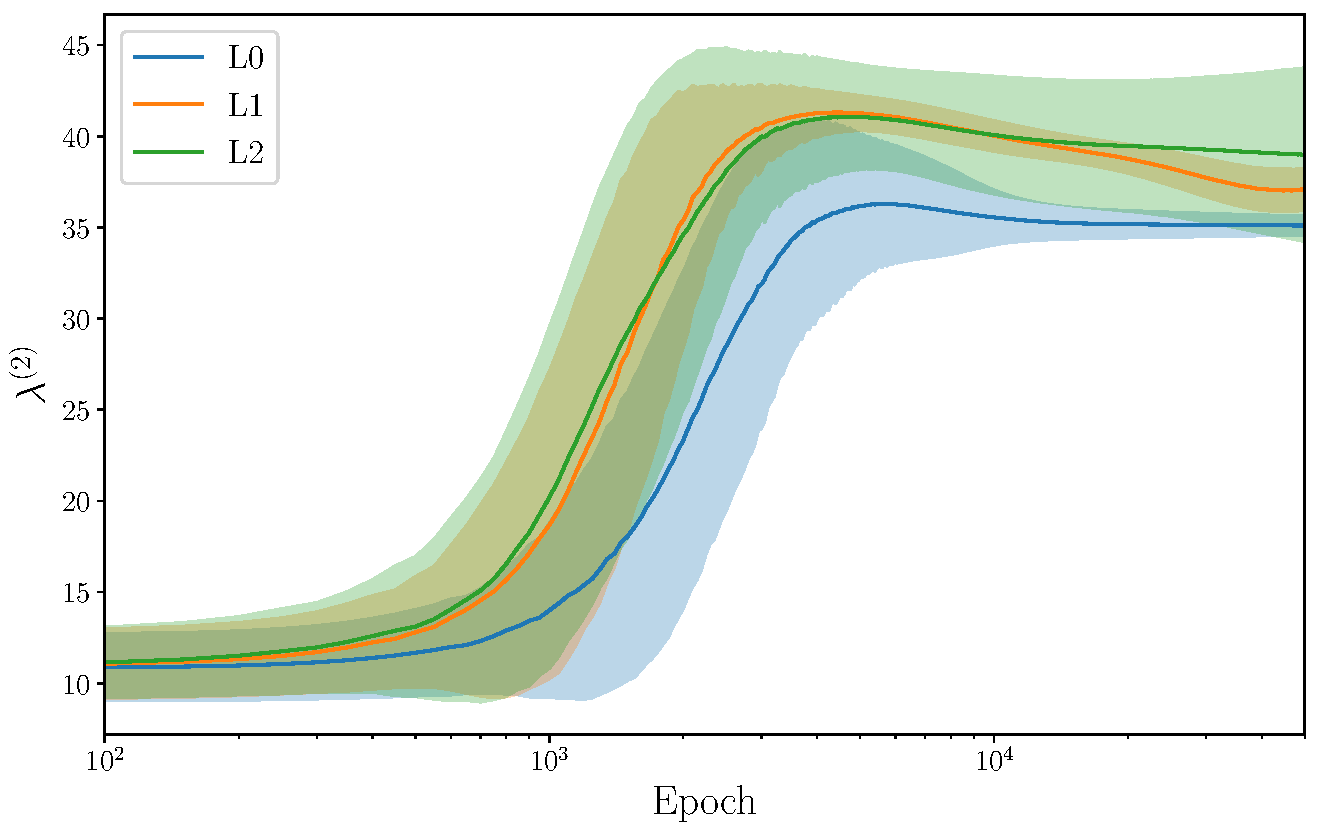
\includegraphics[width=0.30\textwidth]{figs/section_3/ntk_eigvals_L0_L1_L2_n_2.pdf}
  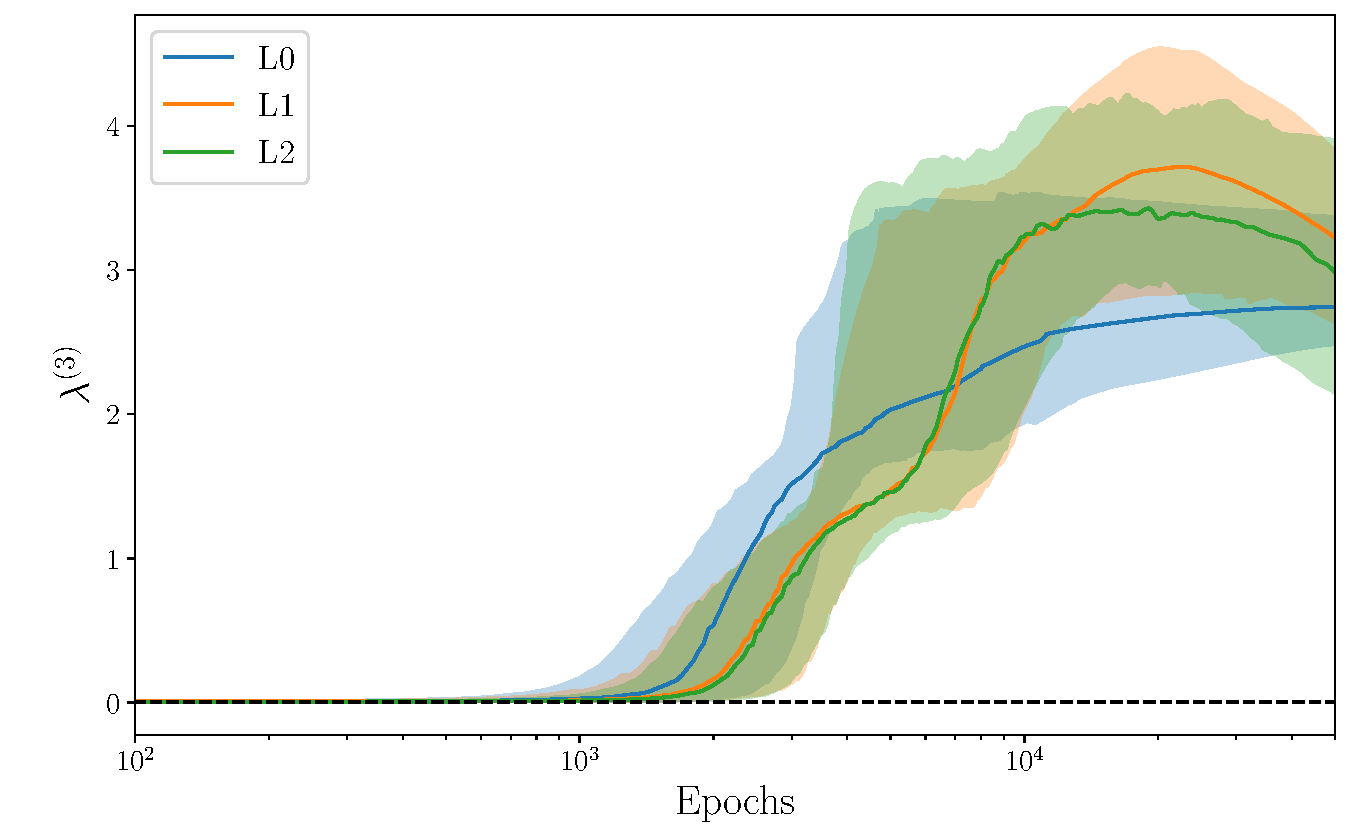
\includegraphics[width=0.30\textwidth]{figs/section_3/ntk_eigvals_L0_L1_L2_n_3.pdf}
  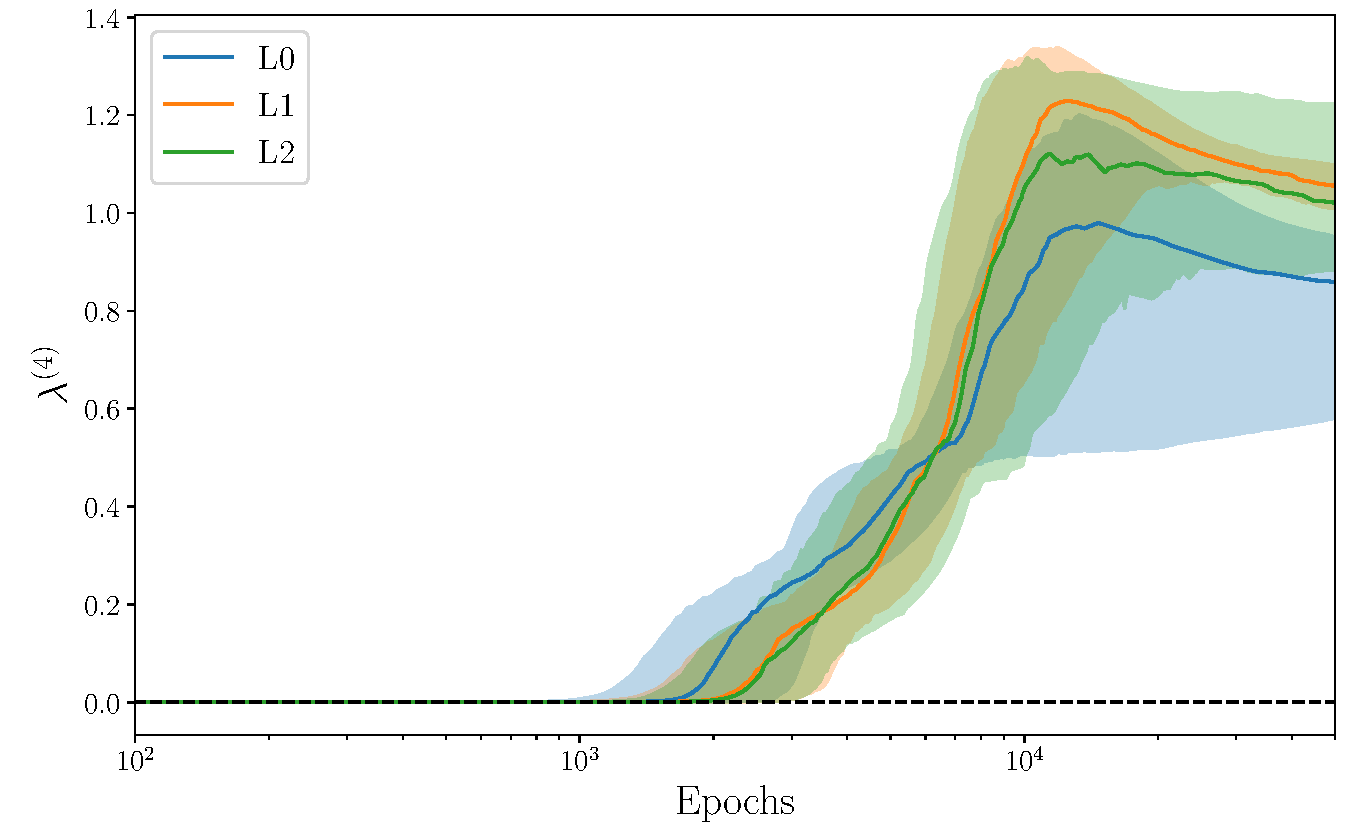
\includegraphics[width=0.30\textwidth]{figs/section_3/ntk_eigvals_L0_L1_L2_n_4.pdf}
  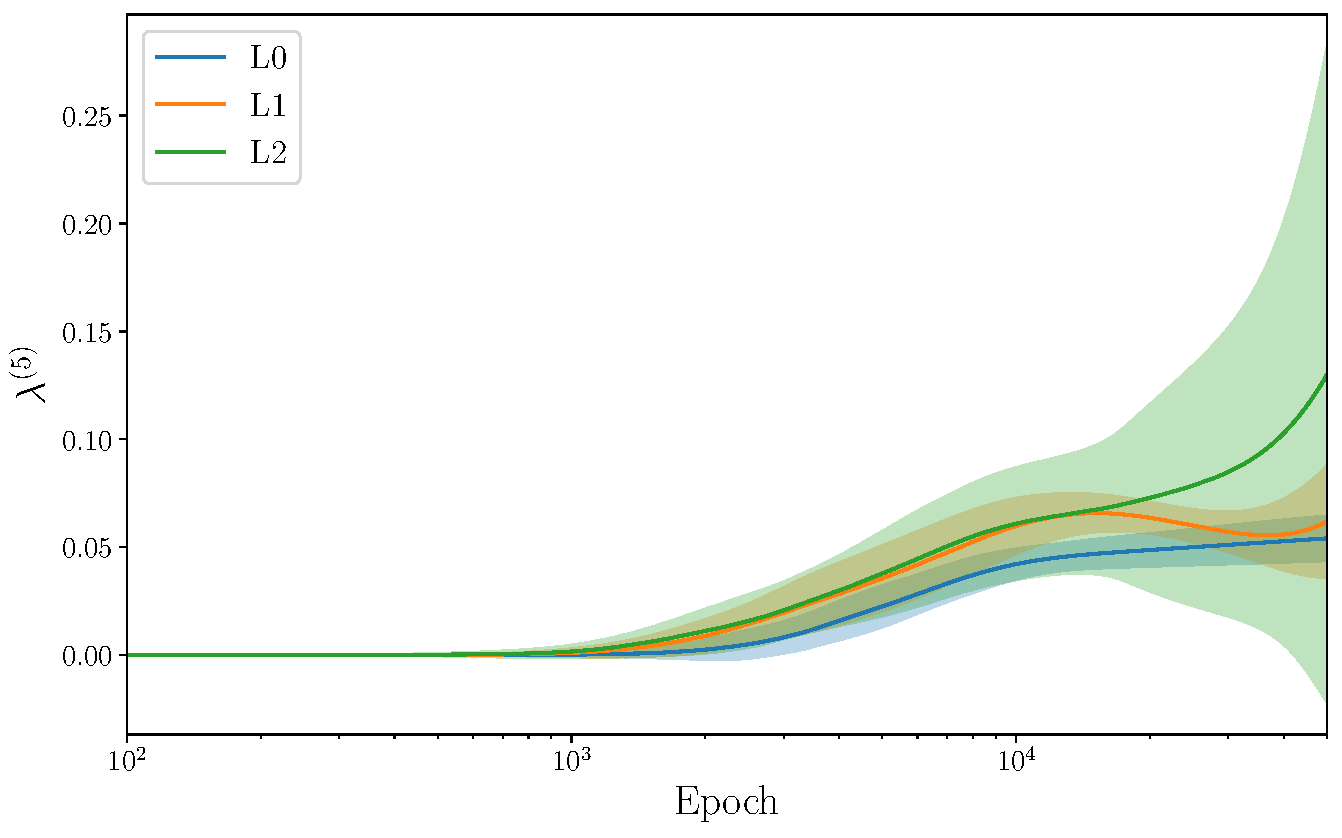
\includegraphics[width=0.30\textwidth]{figs/section_3/ntk_eigvals_L0_L1_L2_n_5.pdf}
  \caption{The first five eigenvalues of the NTK for L0, L1, and L2 data. Solid
  lines represent the median over the ensemble of networks, while solid bands
  correspond to 68\% confidence level.}
  \label{fig:EigvalsComparison}
\end{figure}
% ===================================

In Fig.~\ref{fig:EigvalsComparison}, the same first five eigenvalues of the NTK
are displayed for L0, L1, and L2 data. We observe a common pattern across all
data types, consistently with the observation made before in
Fig.~\ref{fig:NTKTime}. This indicates the the NTK evolution is insensitive to
the noise included in the synthetic data. The increase of the subdominant
eigenvalues, combined with the analysis of Eqs.~\eqref{eq:FlowParallel}
and~\eqref{eq:FlowPerp}, suggests that more ``physical'' features become
learnable before lazy training sets in.

% ===================================
\begin{figure}[t]
  \centering
  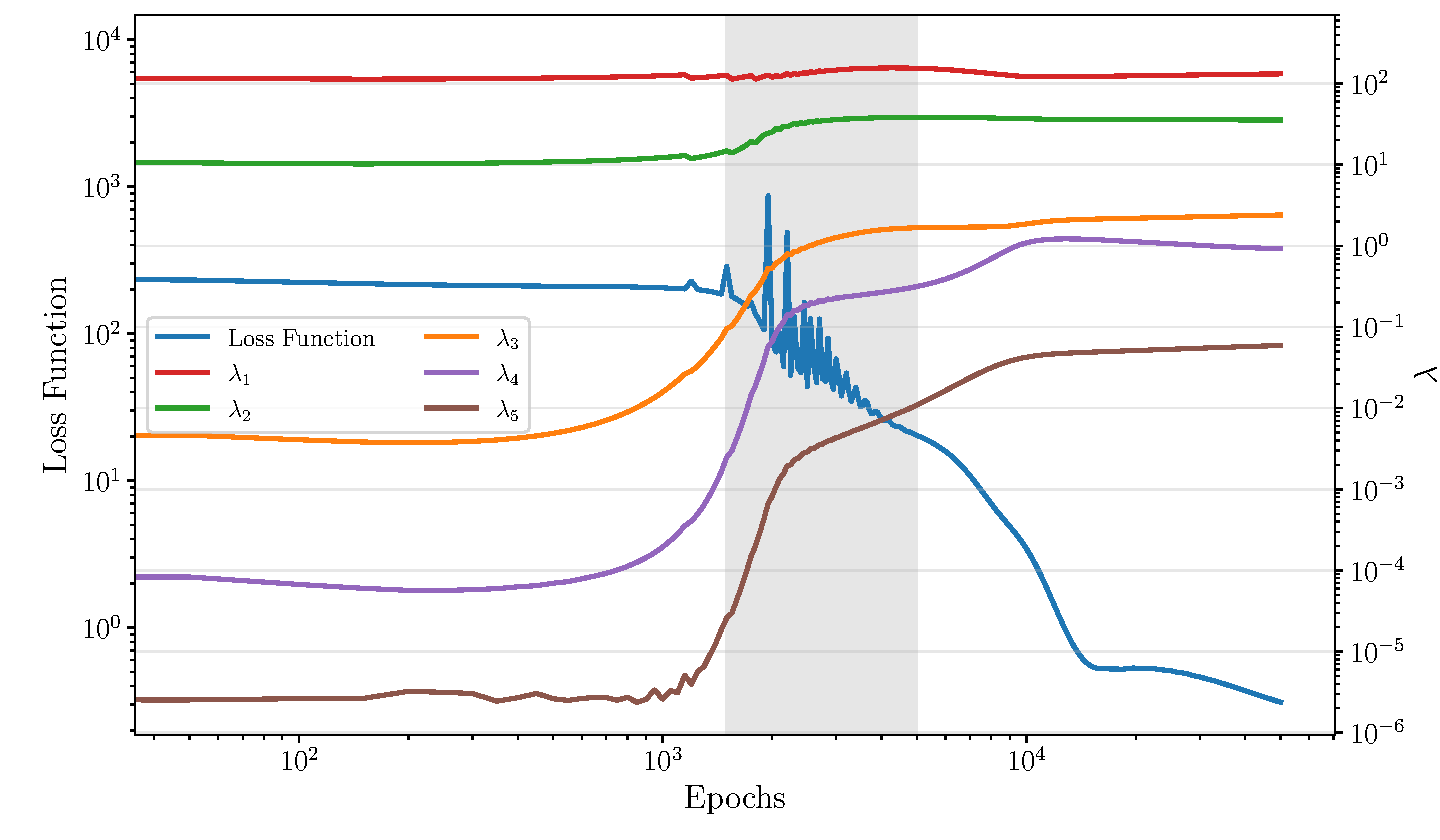
\includegraphics[width=0.30\textwidth]{section_3/loss_and_eigvals_vs_epochs_L0.pdf}
  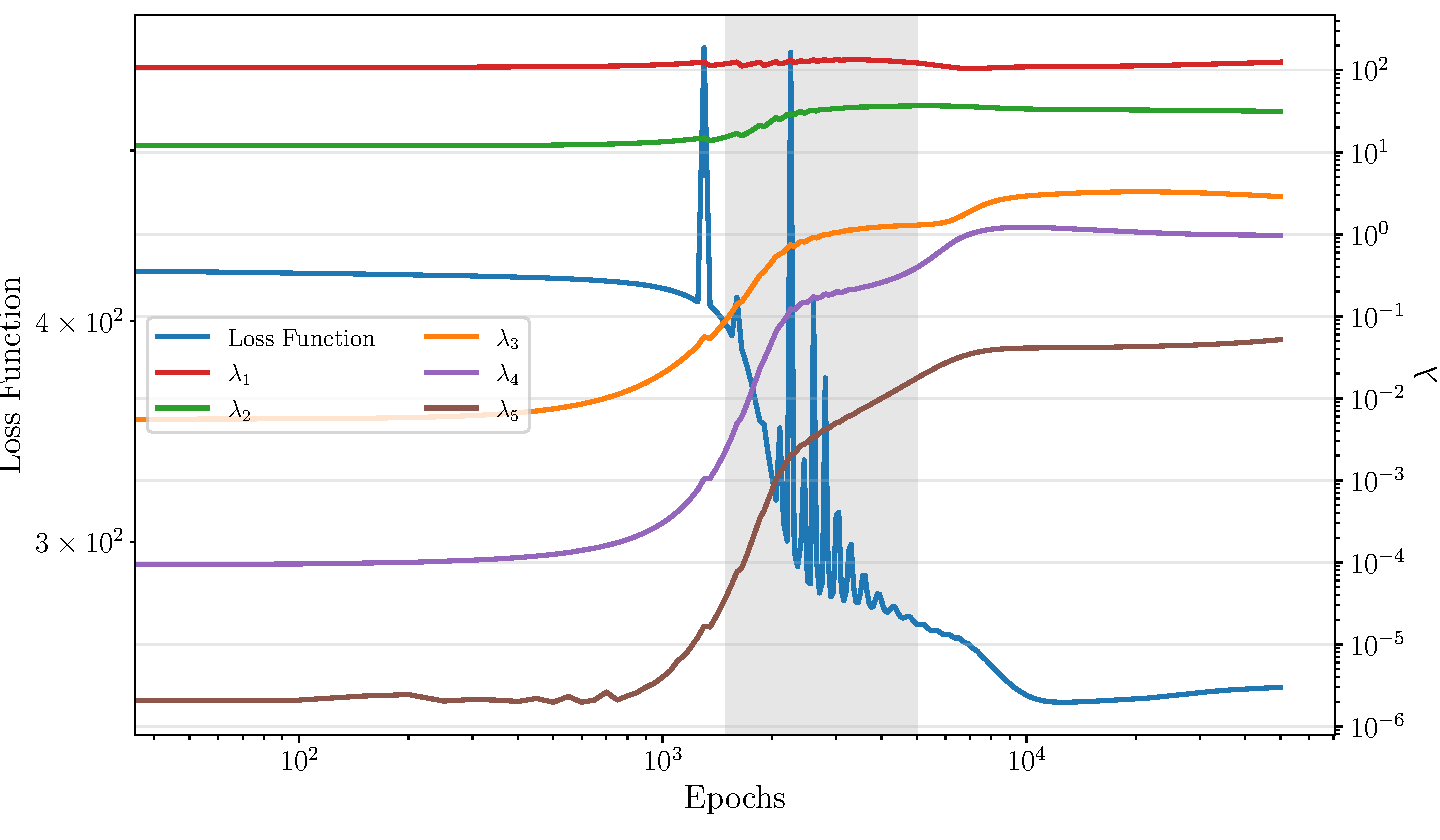
\includegraphics[width=0.30\textwidth]{section_3/loss_and_eigvals_vs_epochs_L1.pdf}
  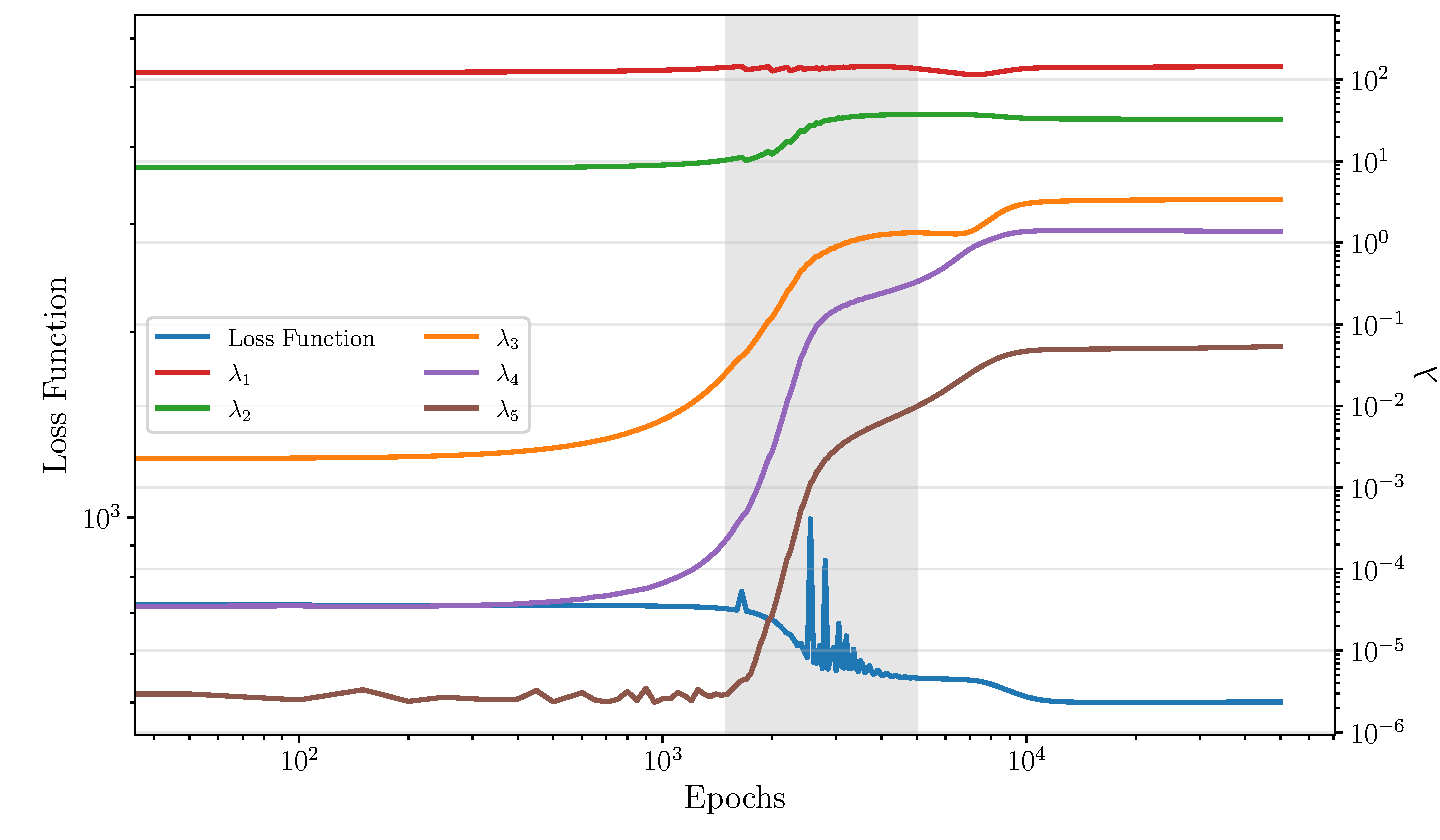
\includegraphics[width=0.30\textwidth]{section_3/loss_and_eigvals_vs_epochs_L2.pdf}
  \caption{Variation of the loss function overlaid with the first five
  eigenvalues for a selected replica over the ensemble using L0 (left), L1
  (center), and L2 (right) data. Left scale refers to the loss, while the right
  scale refers to the eigenvalues.}
  \label{fig:Loss}
\end{figure}
% ===================================

\paragraph{Connection with the loss function} Finally, in Fig.~\ref{fig:Loss} we
show the variation of the loss function during training, overlaid with the first
five eigenvalues of the NTK, for a selected replica over the ensemble. It is
interesting to see that in correspondence with the sudden variation of the
subdominant eigenvalues, the loss function drops significantly, at the cost of
an instability localised in the descent. We interpret this as the network
learning new features, changing its internal representation to accommodate the
new information. After this initial phase, the eigenvalues stabilize and the
loss function decreases smoothly, as expected in the lazy training regime.

As it will be extensively discussed later in Sec.~\ref{sec:LazyTraining}, the
eigenvalues and eigenvectors of the NTK play a special role. Indeed, the output
$f$ can be decomposed into the basis of eigenvectors of the NTK. Hence the
eigenvectors corresponding to the larger eigenvalues can be interpreted as {\em
learnable}\ features, while the small (or zero) eigenvalues correspond to
directions in which the field $f$ never evolves during training.

% \FloatBarrier

\subsubsection{Eigenvectors and Alignment of the NTK}
\label{sec:NTKAlign}

It has been argued before that there is a non-trivial interplay between the
eigenspace of the NTK and that of the matrix $M$. Indeed, the former encodes the
model dependence, while the latter brings physical information. Of course the
two matrices are independent at initialisation, and we do not expect any
alignment pattern between the two. However, this picture may change during
training, as the NTK evolves and the model learns the target function. To
quantify this alignment, we define the matrix $A$, 
\begin{equation}
  \label{eq:MatrixA}
  A_{kk'} = \left( \left< z^{(k)}, v^{(k')}\right> \right)^2 = \cos^2(\theta_{kk'}) \;,
\end{equation}
where $z^{(k)}$ and $v^{(k')}$ are the $k$-th and $k'$-th eigenvectors of the
NTK and $M$, respectively. The matrix $A$ is thus a measure of the alignment
between the eigenspaces of the two matrices. The rows of the matrix correspond
to the eigenvectors of the NTK, ordered by the value of the corresponding
eigenvalues, with the eigenvectors corresponding to the larger eigenvalues at
the top of the matrix. The columns correspond to eigenvectors of the matrix $M$,
also ordered by the values of the corresponding eigenvalues, with the largest
eigenvalues to the left in this case. In Fig.~\ref{fig:NtkMAlign}, we show the
matrix $A$ at different epochs of the training for L2 data and a single NTK
replica. 
% ===================================
\begin{figure}[ht!]
  \centering
  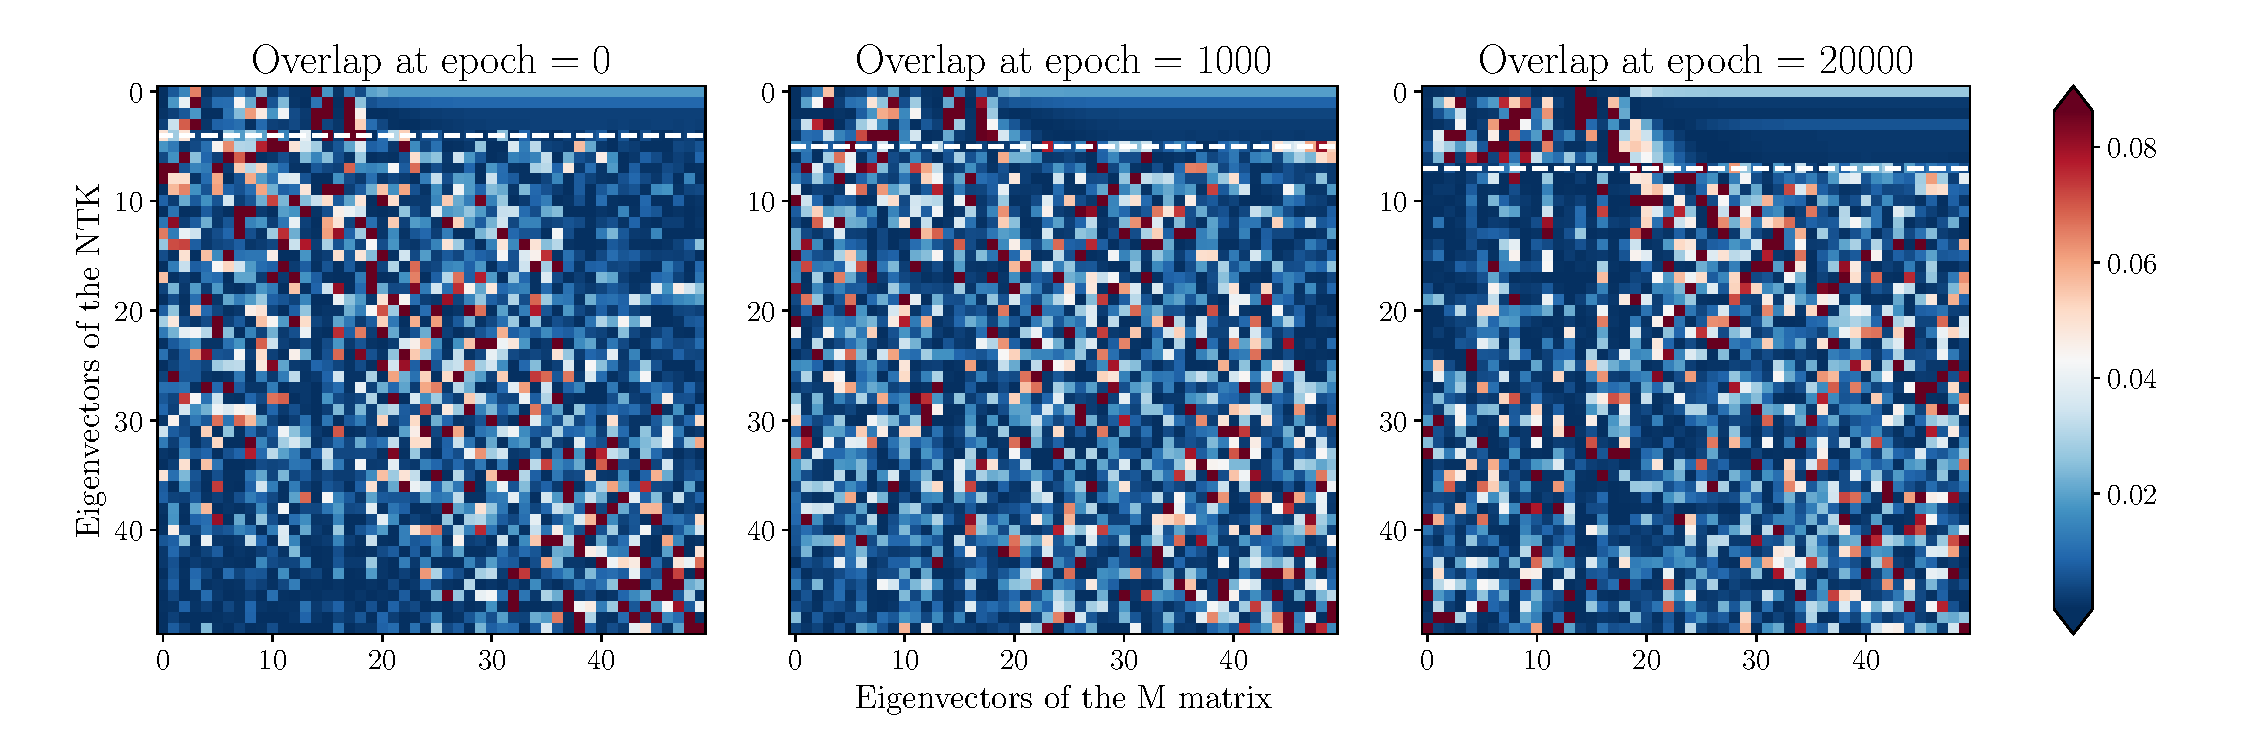
\includegraphics[width=1\textwidth]{section_3/ntk_alignment_L2.pdf}
  \caption{Matrix $A$ as defined in Eq.~\eqref{eq:MatrixA} for L2 data and for a
  single replica of the NTK. The matrix is shown at different epochs of the
  training process, indicated in the top of each panel. The white dashed line
  indicates the cut-off tolerance that we imposed to the eigenvalues of the NTK
  (see Appendix~\ref{app:cutoff}).}
  \label{fig:NtkMAlign}
\end{figure}
% ===================================

% ===================================
\begin{figure}[ht!]
  \centering
  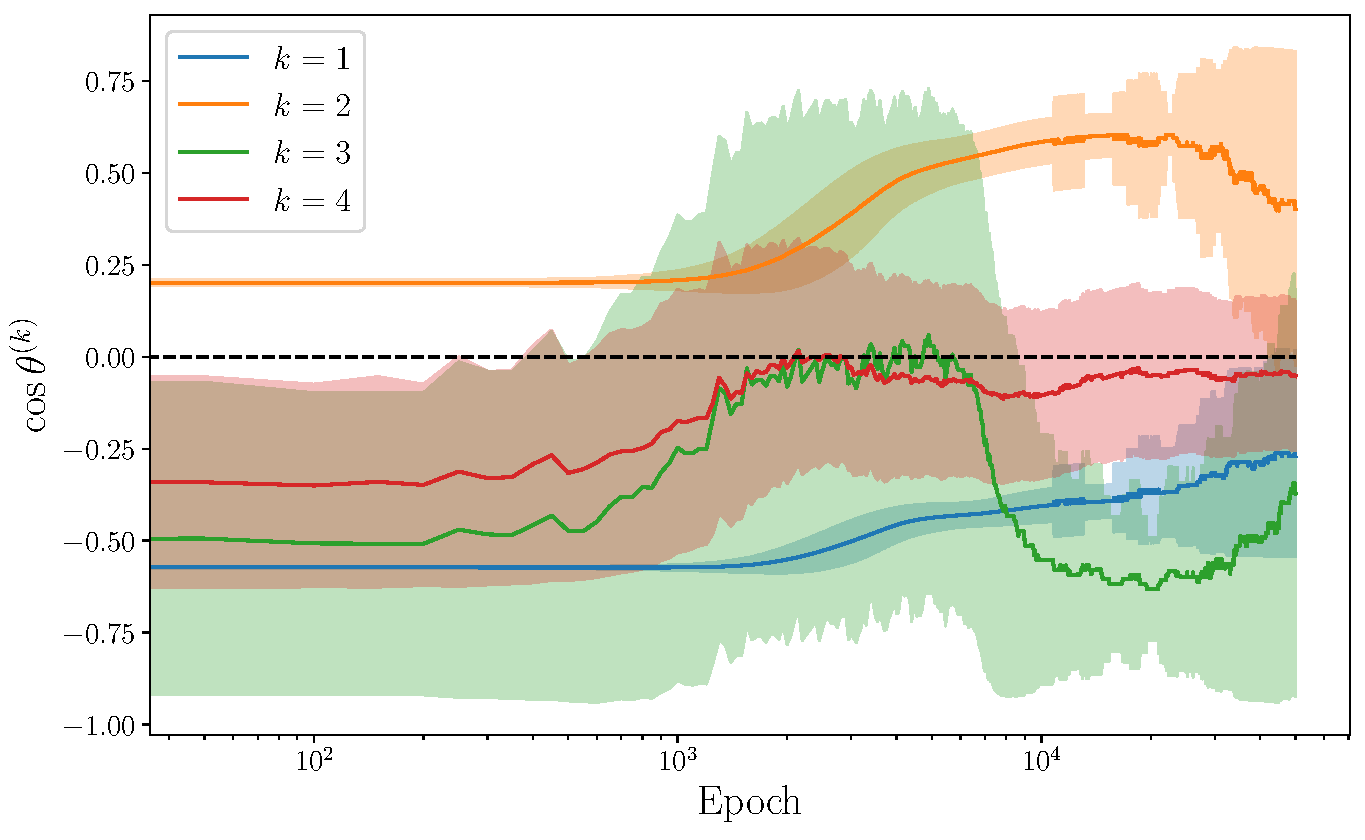
\includegraphics[width=0.45\textwidth]{section_3/ntk_alignment_fin_L2_1}
  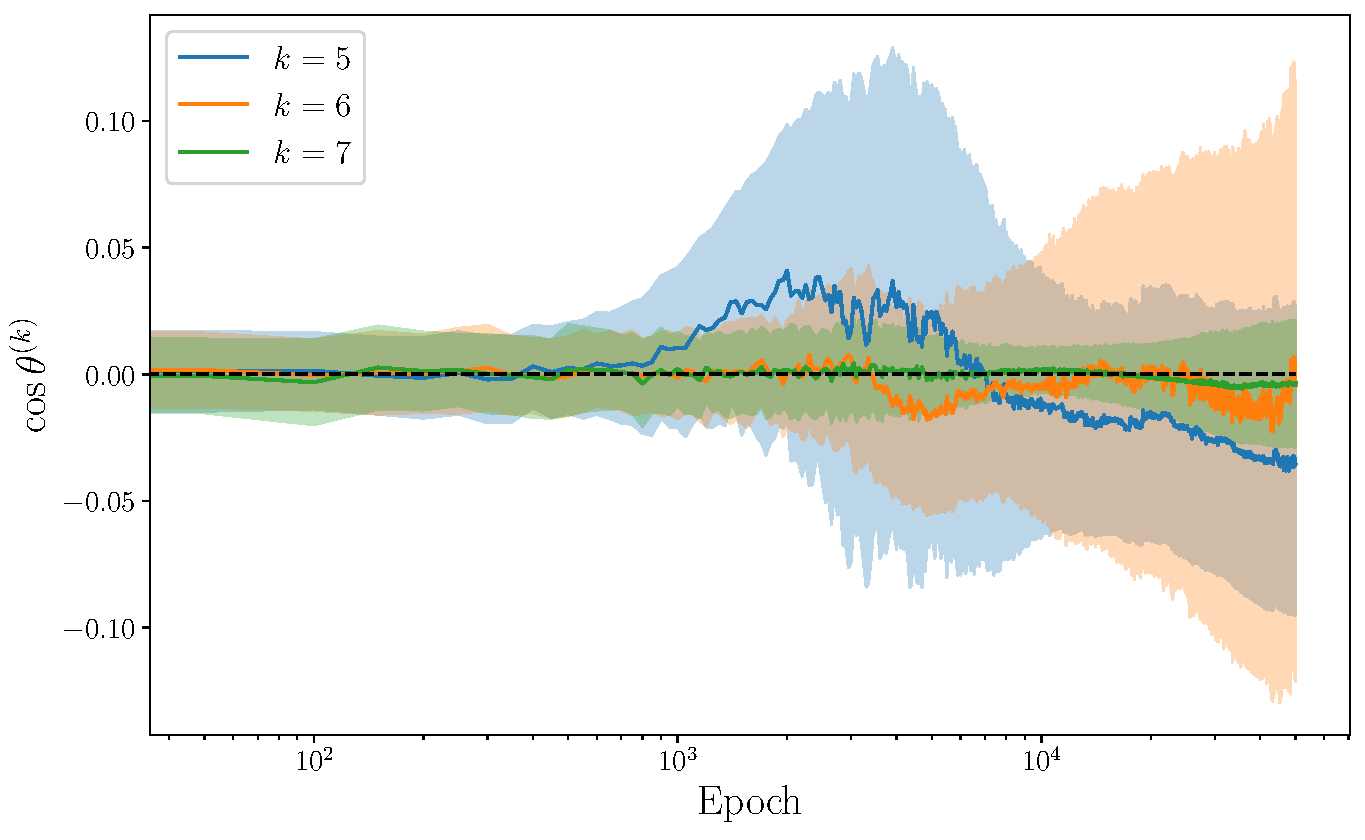
\includegraphics[width=0.45\textwidth]{section_3/ntk_alignment_fin_L2_2}
  \caption{Alignment of the eigenvectors of the NTK with the input function
  $f^{\rm(in)}$ used to generate the L2 data, measured in terms of $\cos
  \theta^{(k)} = (z^{(k)}, f^{\rm{(in)}})/ \Vert f^{\rm{(in)}}\Vert$. In the
  left panel, the first five eigenvectors of the NTK are shown, while the right
  panel shows the remaining eigenvectors up to $k=7$.}
  \label{fig:NTKAlignFin}
\end{figure}
% ===================================
% ===================================
\begin{figure}[ht!]
  \centering
  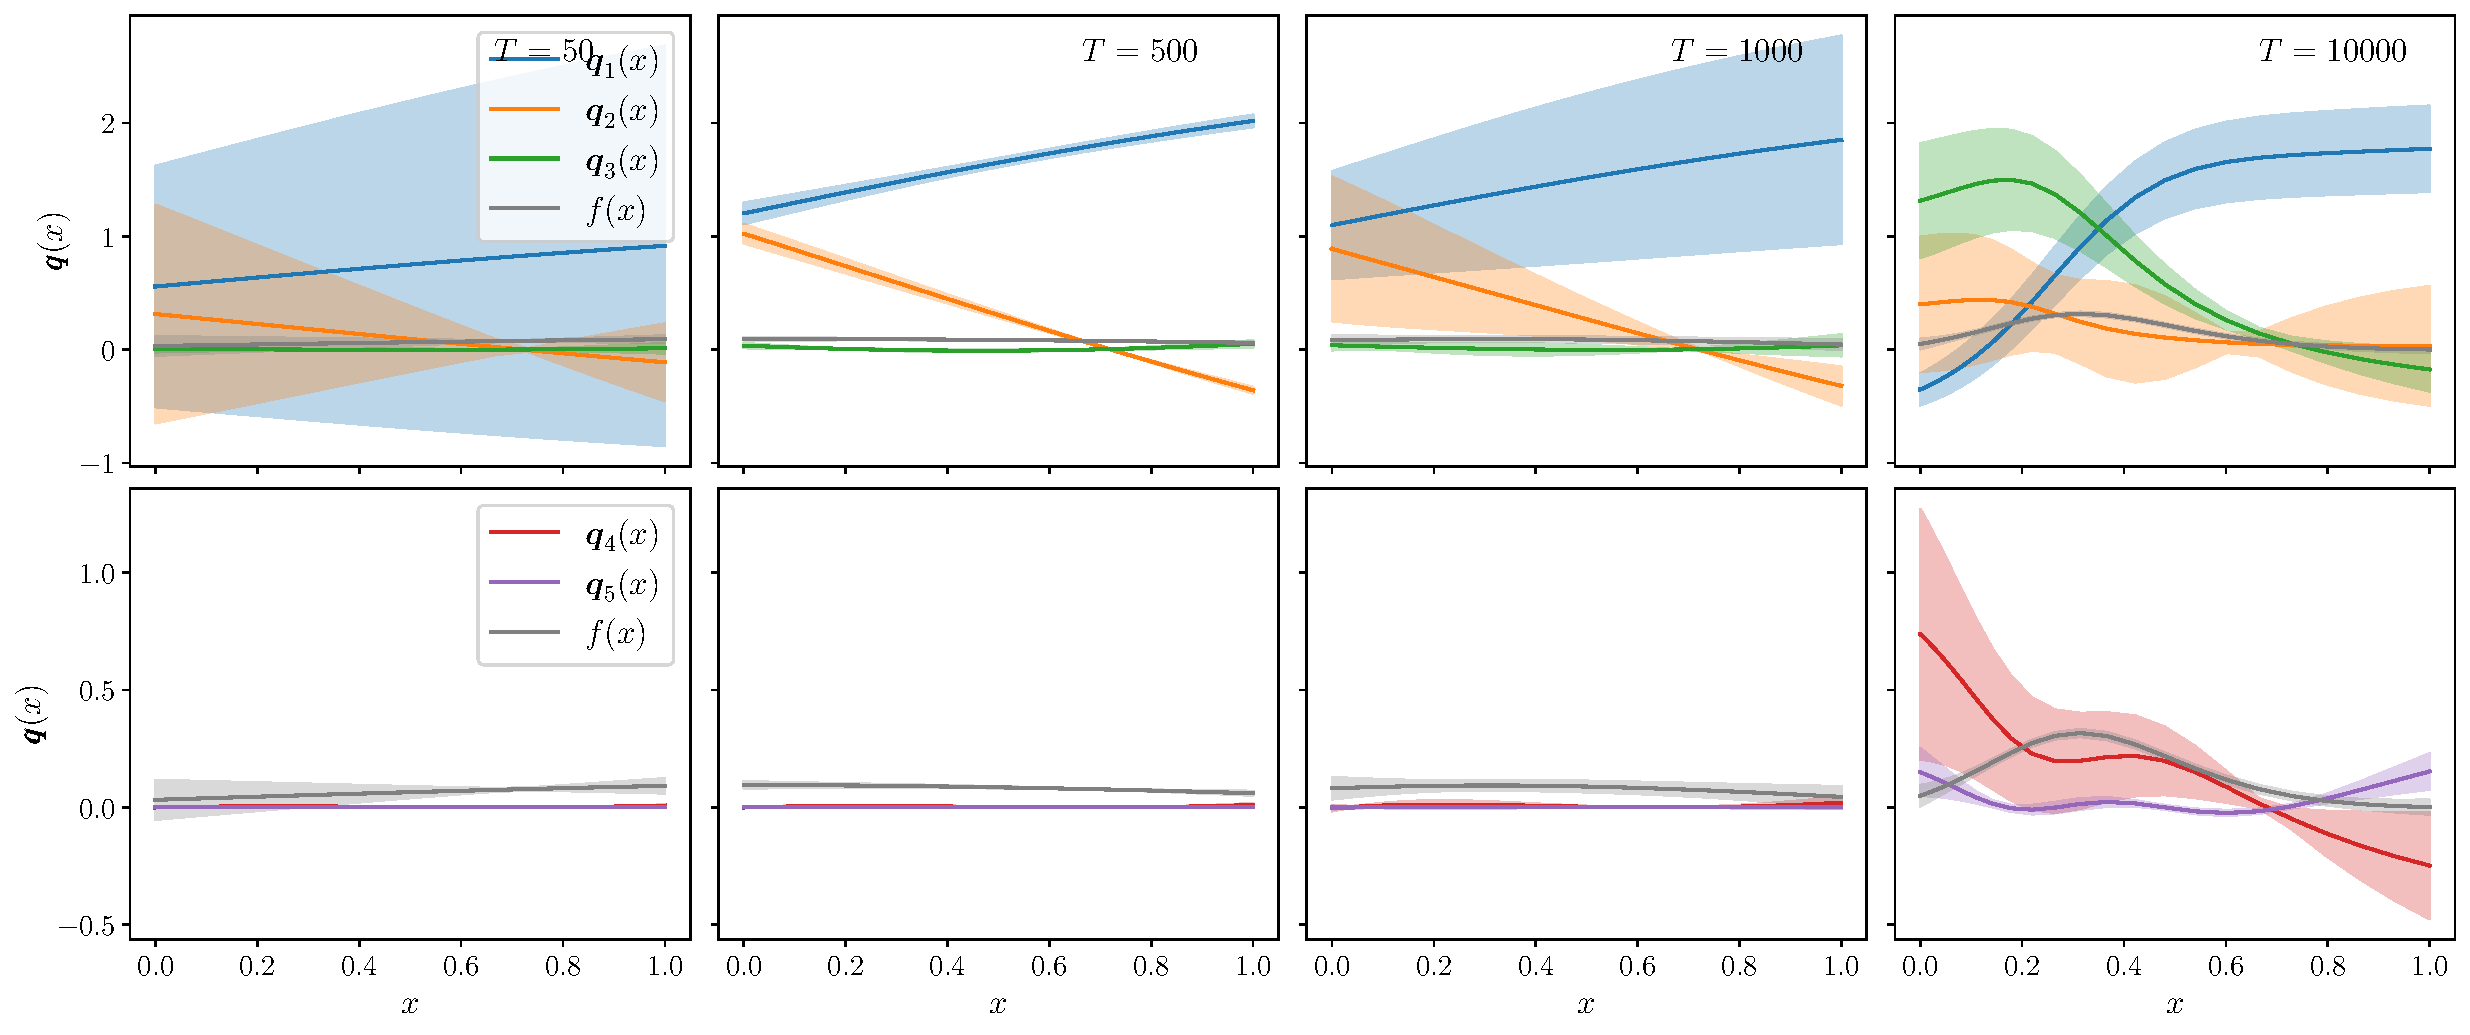
\includegraphics[width=0.90\textwidth]{section_3/q_directions_sign.pdf}
  \caption{First five eigenvectors of the combined matrix $H=\Theta M$, as in
  Eq.~\eqref{eq:FlowEquationNoIndices}, at different training time and as
  function of the input $x$-grid. We also show the output of the network at the
  same training time, which is displayed in gray. L1 data is used. \ac{Should we use L0
  data instead?}}
  \label{fig:NTKMEigVecs}
\end{figure}
% ===================================

The blue rectangle in the top right corner of the matrix shows that the
eigenvectors of the NTK corresponding to the largest eigenvalues are orthogonal
to the eigenvectors of $M$ that are in the kernel of $M$, \ie\ the directions
that do not contribute to the observables. It is useful to remember that the
largest eigenvalues of the NTK correspond to the directions that are orthogonal
to $\ker\Theta$, \ie\ the directions that are learnable during the training
process. In order to have a robust training process, we expect these learnable
directions to align with the directions that actually contribute to the loss
functions, \ie\ the ones corresponding to the largest eigenvalues of $M$.
Consistently with this intuition, we see that the size of this blue rectangle
increases with training time. In particular, it is clear from our plot that it
becomes deeper by the onset of the lazy training regime: more of the learnable
directions -- the {\it features}\ that the network can learn -- are aligned with
the directions that contribute most to the observables.

A similar analysis can also be performed by studying the alignment of the
eigenvectors of the NTK with the input function used to generate the data. In
Fig.~\ref{fig:NTKAlignFin}, we show the cosine of the angle between the two
vectors for two subsects of eigenvectors, in the right and left panel
respectively. In these two panels, different patterns can be observed. First,
the first four angles vary considerably during training, consistent with the
observations made in the figures before. Furthermore, we see that other than
changing the dominant eigenvectors, the NTK is also activating the other
directions that were subdominant in the first stage of training. This in
accordance to what has been previously observed in
Figs.~\ref{fig:EigvalsComparison}-\ref{fig:NtkMAlign}. 

A complementary picture is displayed in Fig.~\ref{fig:NTKMEigVecs}. Here, we
show the eigenvectors of the product of matrices $\Theta M$, labelled with
$q^{(i)}$, at different training times and as functions of the $x$-grid. The
product of these two matrices will become relevant in
Sec.~\ref{sec:LazyTraining}. Together with the eigenvectors, we also show the
output of the trained neural network at the corresponding training time. From
these plots, we see that as the training progresses, the shape of the eigenvectors
become more structured in order to reproduce the output function. Again, this
conclusion supports the observations made previously in various occasions, that
during training the neural network is changing its internal representation and
the NTK encodes this information.

\FloatBarrier
